\documentclass[a4paper]{article}
\usepackage[spanish]{babel}
\usepackage[utf8]{inputenc}
\usepackage{graphicx}
\usepackage{pdfpages}
\usepackage{enumerate}
\usepackage{listings}
\usepackage{color}
\usepackage{indentfirst}
\usepackage{fancyhdr}
\usepackage{latexsym}
\usepackage[colorlinks=true, linkcolor=black]{hyperref}
\usepackage{wrapfig}
\usepackage{calc}
\usepackage{amsmath, amsthm, amssymb}
\usepackage{amsfonts}
\definecolor{gray}{gray}{0.5}
\definecolor{light-gray}{gray}{0.95}
\definecolor{orange}{rgb}{1,0.5,0}

\usepackage{fancyhdr}
\pagestyle{fancy}

%\renewcommand{\chaptermark}[1]{\markboth{#1}{}}
\renewcommand{\sectionmark}[1]{\markright{\thesection\ - #1}}

\fancyhf{}

\fancyhead[LO]{Sección \rightmark} % \thesection\
\fancyfoot[LO]{\small{Leandro Matayoshi, Matías Pizzagalli, Gastón Requeni, Martín Santos}}
\fancyfoot[RO]{\thepage}
\renewcommand{\headrulewidth}{0.5pt}
\renewcommand{\footrulewidth}{0.5pt}
\setlength{\hoffset}{-0.8in}
\setlength{\textwidth}{16cm}
%\setlength{\hoffset}{-1.1cm}
%\setlength{\textwidth}{16cm}
\setlength{\headsep}{0.5cm}
\setlength{\textheight}{25cm}
\setlength{\voffset}{-0.7in}
\setlength{\headwidth}{\textwidth}
\setlength{\headheight}{13.1pt}

\renewcommand{\baselinestretch}{1.1}  % line spacing


\usepackage{underscore}
\usepackage{caratula}
\usepackage{url}

\newcommand{\cod}[1]{{\tt #1}}
\newcommand{\negro}[1]{{\bf #1}}
\newcommand{\ital}[1]{{\em #1}}
\newcommand{\may}[1]{{\sc #1}}
\newcommand{\tab}{\hspace*{2em}}

\newcommand{\sprintstory}[6]{\begin{tabular}{| p{3cm} | p{12cm} |}
 \hline
 TargetProcess ID: & #1 \\
 \hline
 User Story: & #2 \\
 \hline
 Esfuerzo estimado: & #3 \\
 \hline
 Business Value: & #4 \\
 \hline
 Descripción: & #5 \\
 \hline
 Criterios de\newline Aceptación: & #6 \\
 \hline
\end{tabular}}

\newcommand{\simplestory}[5]{\begin{tabular}{| p{3cm} | p{12cm} |}
 \hline
 TargetProcess ID: & #1 \\
 \hline
 User Story: & #2 \\
 \hline
 Esfuerzo estimado: & #3 \\
 \hline
 Business Value: & #4 \\
 \hline
 Descripción: & #5 \\
 \hline
\end{tabular}}

\newenvironment{taskstable}
{ \begin{tabular}{| p{14cm} | p{1cm} |}
 \hline
 \multicolumn{2}{|c|}{{\bf División en tareas}}\\
 \hline
 {\bf Tarea} & {\bf HH}\\
 \hline }
{ \end{tabular} }

\newcommand{\task}[2]{#1 & #2\\
 \hline}

\hypersetup{
 pdfstartview= {FitH \hypercalcbp{\paperheight-\topmargin-1in-\headheight}},
 pdfauthor={Grupo},
 pdfsubject={Dise\~{n}o}
}

\lstset{escapechar=@}

\begin{document}

\thispagestyle{empty}
\materia{Ingeniería de Software II}
\submateria{Primer Cuatrimestre de 2016}
\titulo{Trabajo Práctico I: The Curry Game}

\integrante{Leandro Matayoshi}{79/11}{leandro.matayoshi@gmail.com}
\integrante{Matías Pizzagalli}{257/12}{matipizza@gmail.com}
\integrante{Gastón Requeni}{400/11}{grequeni@hotmail.com}
\integrante{Martín Santos}{413/11}{javiersm00@gmail.com}

\makeatletter

\maketitle

\newenvironment{myindentpar}[1]
{\begin{list}{1}
         {\setlength{\leftmargin}{#1}}
         \item[]
}
{\end{list}}

\newpage
\section{Primera parte de la entrega}
\subsection{Introducción}
Aca va la intro =)

\subsection{Estimación de Esfuerzo}
Una vez construidas las user stories, empezamos a estimar el esfuerzo en story points. Para esto utilizamos la técnica de Planning Poker.

Primero realizamos la estimación de las historias asociadas al simulador. Cada integrante del equipo eligió un conjunto de historias 
que consideró de 1 punto de esfuerzo. Luego realizamos una puesta en común en la que estuvimos de acuerdo por unanimidad. A continuación
analizamos todas las tarjetas restantes relacionadas con la simulación y acordamos un puntaje utilizando Planning Poker. La técnica
fue muy útil para llegar a un acuerdo, ya que permitió evaluar posturas muy distintas sobre las historias. En algunos casos hubo acuerdos casi
unánimes y en otros dedicamos bastante tiempo a la discusi\'on.

Luego estimamos las historias por fuera del simulador. También comenzamos eligiendo una con esfuerzo de 1 punto y a partir de esa estimamos
el resto hasta completar el proceso.
\subsection{Estimación de Business Value}
El valor de cada story fue calculado en función de su importancia dentro del sistema. 

Dentro de las stories con más valor se distinguen 2 grandes grupos:
\begin{itemize}
  \item Aquellas relacionadas con el simulador, ya que como fue mencionado anteriormente es prioritario para el cliente
  \item Aquellas indispensables para la aplicación, sin las cuales la misma deja de tener sentido. En este caso temas de registro y login de usuarios y creación y aceptación
  de desafíos
\end{itemize}

En el nivel de \emph{great} incluímos aquellas que le dan identidad y flexibilidad a nuestro juego. En este caso, relacionadas con las apuestas de fichas en los desafíos,
y las restricciones de capital a la hora de armar los equipos.

Las stories calificadas como \emph{good} son similares a las de \emph{great} pero de menor importancia.


\newpage
\subsection{Project Backlog}
%%%%% EJEMPLOS DE USER STORY DE BACKLOG

% \simplestory
% {1}
% {Como usuario no registrado quiero ingresar mi nombre, mi cuenta de email y una contraseña para poder registrarme en la aplicación.}
% {3 pt.}
% {Nice to Have}
% {-}

%%%%%%%%%%%%%%%%%%%%%%%

\simplestory
{1}
{Como diseñador del juego quiero que se obtengan datos de popularidad en Twitter de los jugadores para afectar las fórmulas de umbral de éxito.}
{13 pt.}
{Nice to Have}
{Los datos tienen que obtenerse durante la simulación del partido y en lo posible tener en cuenta si son positivos o negativos.}

\vspace{1cm}

\simplestory
{2}
{Como participante quiero armar un equipo de basket para utilizarlo en desafíos.}
{3 pt.}
{Must Have}
% No queda muy lindo el itemize adentro de la tabla...
{\begin{itemize}
\item El equipo debe tener 5 jugadores (base, escolta, alero, ala pivot, pivot) elegidos de una lista con todos los jugadores de la liga.
\item Cada jugador de la lista permitirá acceder a su costo (valor ficticio) y a sus estadísticas.
\item Se deberá validar que no se supere el cap.
\end{itemize}}

\vspace{1cm}

\simplestory
{3}
{Como administrador del equipo quiero elegir el técnico que dirige a mi equipo para personalizar mi equipo y determinar las posibles estrategias ofensivas y defensivas.}
{2 pt.}
{Must Have}
{\begin{itemize}
\item Elegir técnico de una lista con todos los técnicos existentes en la liga.
\item Ver jugadas que tiene asociadas cada técnico.
\end{itemize}}

\vspace{1cm}

\simplestory
{4}
{Como diseñador del juego quiero cargar jugadores y sus datos estadísticos manualmente para que haya jugadores en el sistema.}
{3 pt.}
{Average}
{\begin{itemize}
\item Los porcentajes FG y 3P deben estar entre 0 y 100, APG $>=$ 0, RPG $>=$ 0, BPG $>=$ 0, SPG $>=$ 0, TO $>=$ 0, PPG $>=$ 0.
\item Se ingresan los jugadores uno por uno.
\end{itemize}}

\vspace{1cm}

\simplestory
{5}
{Como diseñador del juego quiero crear técnicos asociándolos con un libro de jugadas para que haya técnicos en el sistema}
{2 pt.}
{Average}
{-}

\vspace{1cm}

\simplestory
{6}
{Como administrador del equipo quiero ingresar un nombre para mi equipo para personalizar mi equipo.}
{1 pt.}
{Good}
{-}

\vspace{1cm}

\simplestory
{7}
{Como participante quiero guardar un equipo creado en mi lista de equipos para utilizarlo en desafíos posteriores.}
{1 pt.}
{Good}
{-}

\vspace{1cm}

\simplestory
{8}
{Como participante quiero elegir un equipo de la lista para utilizarlo en el desafìo actual.}
{1 pt.}
{Good}
{-}

\vspace{1cm}

\simplestory
{9}
{Como participante quiero ver tabla de posiciones en base a cantidad de fichas ganadas en apuestas para compararse con otros participantes.}
{2 pt.}
{Good}
{-}

\vspace{1cm}

\simplestory
{10}
{Como participante quiero ver tabla de posiciones en base a desafíos ganados/perdidos para compararse con otros participantes.}
{2 pt.}
{Good}
{-}

\newpage
\subsection{Sprint Backlog}
%%%%% EJEMPLOS DE USER STORY Y TAREAS

% \sprintstory
% {1}
% {Como usuario no registrado quiero ingresar mi nombre, mi cuenta de email y una contraseña para poder registrarme en la aplicación.}
% {3 pt.}
% {Nice to Have}
% {-}
% {\begin{itemize}
%   \item Ingresar mi nombre, mi cuenta de email y una contraseña, y apretar un botón que confirme el registro.
%   \item No debe permitir ingresar un mail sintácticamente inválido.
%   \item No debe permitir registrar dos veces el mismo mail.
%   \item La contraseña debe ser ingresada dos veces y el sistema validar que sean idénticas.
% \end{itemize}}

% \vspace{1cm}

% \begin{taskstable}
%  \task
%  {Como usuario no registrado quiero ingresar mi nombre, mi cuenta de email y una contraseña para poder registrarme en la aplicación}
%  {3}

%  \task
%  {Como usuario no registrado quiero ingresar mi nombre, mi cuenta de email y una contraseña para poder registrarme en la aplicación}
%  {3}
% \end{taskstable}

%%%%%%%%%%%%%%%%%%%%%%%%%%%%%%%%%%%%%%%%%%%%%%%%%%%%%%%%%%%%%%%%%%%%%%%%%%%%%%%%%%%%%%%%%%%%%



\newpage
\section{Segunda parte de la entrega}
\subsection{Seguimiento del Sprint}
El Sprint realizado entre el 12/04/2016 y el 04/05/2016 se completó exitosamente. Todas las user stories planificadas fueron terminadas.
A continuación presentamos los burndown charts asociados y el detalle de horas consumidas:

\begin{figure}[h!]
 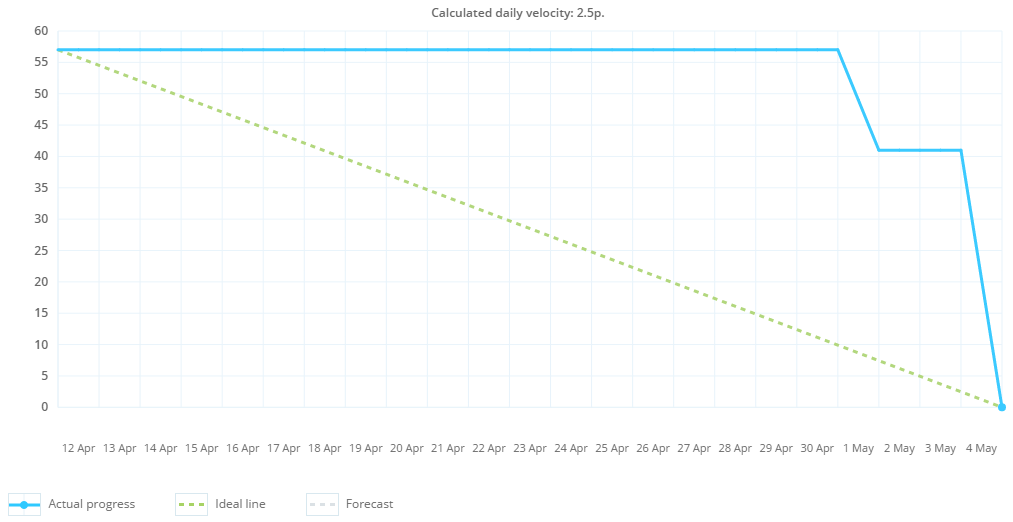
\includegraphics[width=\textwidth]{imagenes/burndown-points.png}
 \caption{Burndonw Chart de Story Points. La línea verde punteada indica el progreso ideal (comienza en 57 puntos, el total de la estimación de esfuerzo).
 La línea azul indica el progreso real.}
\end{figure}

\begin{figure}[h!]
 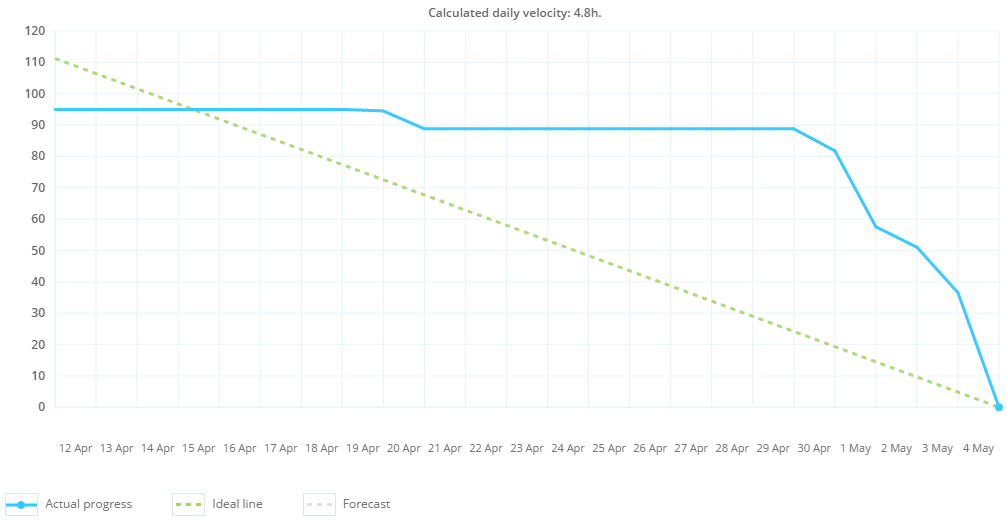
\includegraphics[width=\textwidth]{imagenes/burndown-hours.png}
 \caption{Burndonw Chart de Horas de Tareas. La línea verde punteada indica el progreso ideal (comienza en 111 horas, lo cual difiere de la estimación
 inicial de 96 horas porque se agregaron horas durante el sprint). La línea azul indica el progreso real.}
\end{figure}

En los gráficos se observa que hasta el 19/04 no hubo avance. El 20/04 se realizaron algunas tareas para discutir en la reunión con el Product Owner del
21/04. Hasta aquí no se cerró ninguna story (por eso los Story Points se mantienen constantes). En este momento se detectaron fallas en la estimación
y se agregaron horas a las tareas (es por esto que la horas empiezan estando por debajo del total de horas).

Luego hubo otro período sin avances y finalmente
a partir del 30/04 empezó a haber avance contínuo en las tareas. El 1/05 se cerró la primer user story y de ahí en más se fueron cerrando el resto.

Finalmente, la cantidad de horas hombre consumidas fue de:

\vspace{0.3cm}
\begin{tabular}{ | c | c | }
 \hline
 Horas Integrante 1: & 21\\
 \hline
 Horas Integrante 2: & 14\\
 \hline
 Horas Integrante 3: & 33.5\\
 \hline
 Horas Integrante 4: & 29.5\\
 \hline
 {\bf Horas Totales:} & 92.5\\
 \hline
\end{tabular}


\subsection{Retrospectiva}
Los atrasos fueron causados principalmente por las actividades que los integrantes realizamos además de trabajar en este proyecto. Todos
nosotros tenemos trabajos de 6hs diarias. Adem\'as uno de los integrantes dedica 10 hs por semana a la docencia y el resto est\'a cursando otra materia
en la facultad. Haciendo un balance general y teniendo en cuenta horas de descanso, por semana cada uno tuvo disponible aproximadamente 10 horas (sin
contar los fines de semana). Por último hay que tener en cuenta que la coordinación grupal se complicó por la dificultad de coincidir todos en un mismo
horario.

En conclusión, las horas netas que cada uno tuvo disponibles fueron muy pocas (en las 3 semanas del sprint, cada uno tuvo aproximadamente unas 30 hs
disponibles más fines de semana). Además hubo una semana de disponibilidad cero por el parcial, por ende sólo tiene sentido considerar
dos semanas. Esto explica claramente los saltos en los burndowns.

Para llegar a tiempo a la entrega, en el avance del 20/04 se realizó una reunión grupal para pensar un diseño a nivel global y establecer parámetros
en común. Luego se repartieron stories iniciales para cada uno (dos por persona) y se avanzó en la parte central del simulador. Cada uno fue tomando
stories extra a medida que las terminaba o que se veía imposibilitado para avanzar.

Detectamos muchas dependencias entre stories. Esto provocó que en un punto las stories estaban completamente distribuidas pero ninguna había sido
completada porque se necesitaba integración con stories de otra persona. Es por esto que muchas stories se cerraron en los últimos días, mientras
que las horas fueron disminuyendo de manera más gradual.

Al unificar las partes, detectamos ciertos problemas a solucionar en un próximo sprint:
\begin{itemize}
 \item El logger no es cerrado para la modificación cuando se quieran agregar movimientos (por ejemplo: HacerFalta).
 \item Los parámetros deben ser modificados desde la clase que los usa. Esto deberíamos abstraerlo en algúna estructura especial que pueda
 ser modificada sin afectar a los que la usan.
 \item El jugador estrella (MVP) quedó fuera de esta iteración.
 \item Las fórmulas de resolución de acciones solo tienen en cuenta las estadísticas del jugador que lleva a cabo la acción. Por ejemplo, en el caso de un tiro por tres puntos, no tomamos en cuenta la cantidad de pases que se hicieron previamente. Esto es algo a resolver en la siguiente iteracion.
\end{itemize}


\newpage

\bibliographystyle{plain}
\bibliography{tp3}

\end{document}
